\documentclass[a4paper,11pt]{article}

\usepackage[T1]{fontenc}
\usepackage[utf8]{inputenc}
\usepackage{graphicx}
\usepackage{xcolor}

\renewcommand\familydefault{\sfdefault}
\usepackage{tgheros}
\usepackage[defaultmono]{droidmono}

\usepackage{amsmath,amssymb,amsthm,textcomp}
\usepackage{enumerate}
\usepackage{multicol}
\usepackage{tikz}
\usepackage{graphics}
\usepackage{lstlinebgrd}
\usepackage{color}
\usepackage{geometry}
\geometry{total={210mm,297mm},
left=25mm,right=25mm,%
bindingoffset=0mm, top=20mm,bottom=20mm}


\linespread{1.3}

\newcommand{\linia}{\rule{\linewidth}{0.5pt}}

\newtheoremstyle{mytheor}
    {1ex}{1ex}{\normalfont}{0pt}{\scshape}{.}{1ex}
    {{\thmname{#1 }}{\thmnumber{#2}}{\thmnote{ (#3)}}}

\theoremstyle{mytheor}
\newtheorem{defi}{Definition}

% my own titles
\makeatletter
\renewcommand{\maketitle}{
\begin{center}
\vspace{2ex}
{\huge \textsc{\@title}}
\vspace{1ex}
\\
\linia\\
\@author \hfill \@date
\vspace{4ex}
\end{center}
}
\makeatother
%%%

% custom footers and headers
\usepackage{fancyhdr}
\pagestyle{fancy}
\lhead{Page \thepage}
\chead{}
\rhead{Steven Seppala \& Seth Decker}
\lfoot{Programming assignment \textnumero{} 5}
\cfoot{Networks}
\rfoot{ECE 440}
\renewcommand{\headrulewidth}{0pt}
\renewcommand{\footrulewidth}{0pt}
%

% code listing settings
\usepackage{listings}
\lstset{
    language=[ANSI]C,
    basicstyle=\ttfamily\small,
    aboveskip={1.0\baselineskip},
    belowskip={1.0\baselineskip},
    columns=fixed,
    extendedchars=true,
    breaklines=true,
    tabsize=4,
    prebreak=\raisebox{0ex}[0ex][0ex]{\ensuremath{\hookleftarrow}},
    frame=lines,
    showtabs=false,
    showspaces=false,
    showstringspaces=false,
    keywordstyle=\color[rgb]{0.627,0.126,0.941},
    commentstyle=\color[rgb]{0.133,0.545,0.133},
    stringstyle=\color[rgb]{01,0,0},
    numbers=left,
    numberstyle=\small,
    stepnumber=1,
    numbersep=10pt,
    captionpos=t,
    escapeinside={\%*}{*)}
}
	\definecolor{dkgreen}{rgb}{0,0.8,0}
	\definecolor{gray}{rgb}{0.5,0.5,0.5}
	\definecolor{mauve}{rgb}{0.58,0,0.82}

%%%----------%%%----------%%%----------%%%----------%%%
%%%----------Document begins right below this-------%%%
%%%----------%%%----------%%%----------%%%----------%%%
\begin{document}

\title{Lab Problems \textnumero{} 1}

\author{Steven Seppala \& Seth Decker}

\date{30 October 2014}

\maketitle

\begin{center} \section*{Lab Problems} \end{center}

\begin{enumerate}
\item {Problem 3.17} \\
    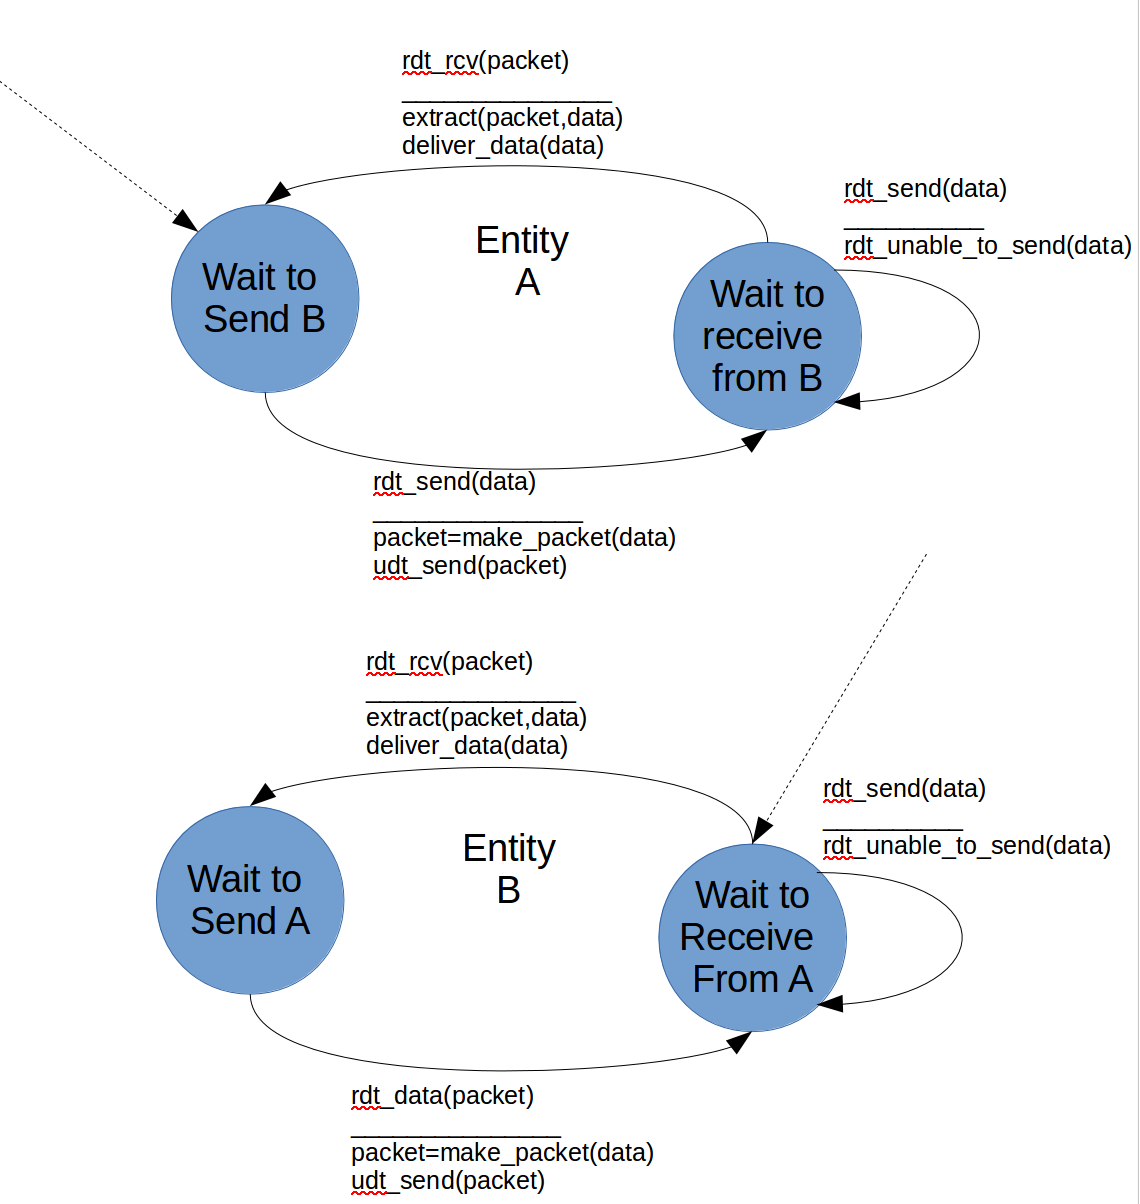
\includegraphics[width=120mm]{p17}
    \pagebreak
\item{Problem 3.18}
    \par
    The sender waits for ACK before it can send the next pair of messages; the ACK messages received will have an ID that dictates which packet was received.\\
    RECIEVER: \\
    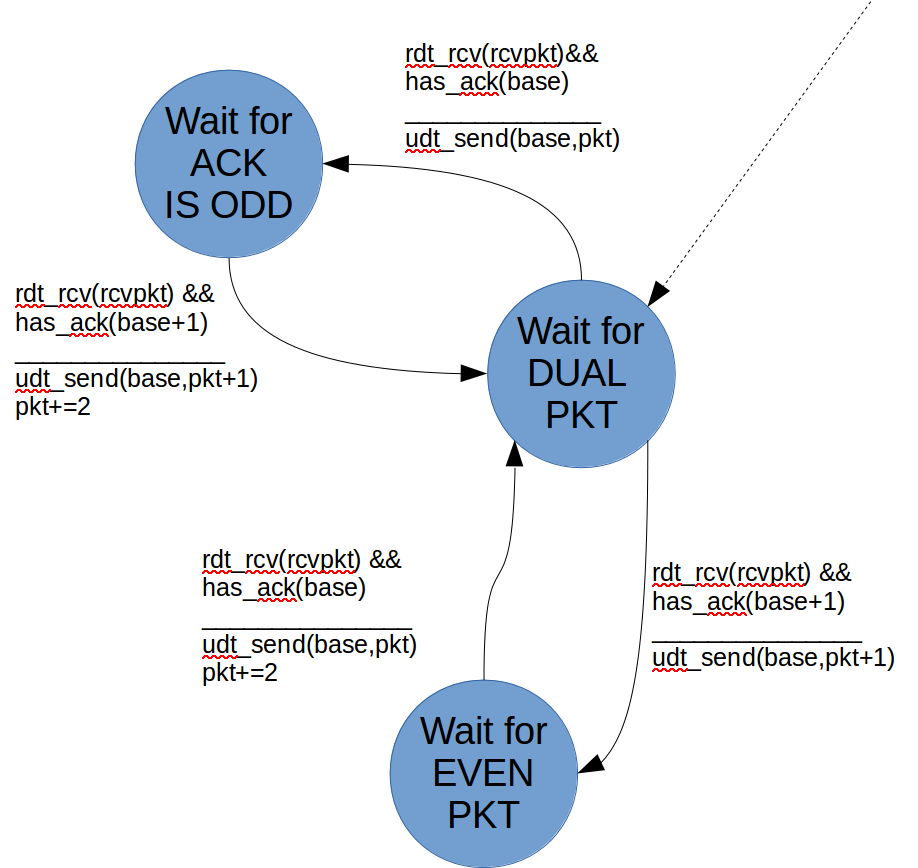
\includegraphics[width=\textwidth]{reciever_18_fsm}\\
    \pagebreak
    \bold{SENDER:}
    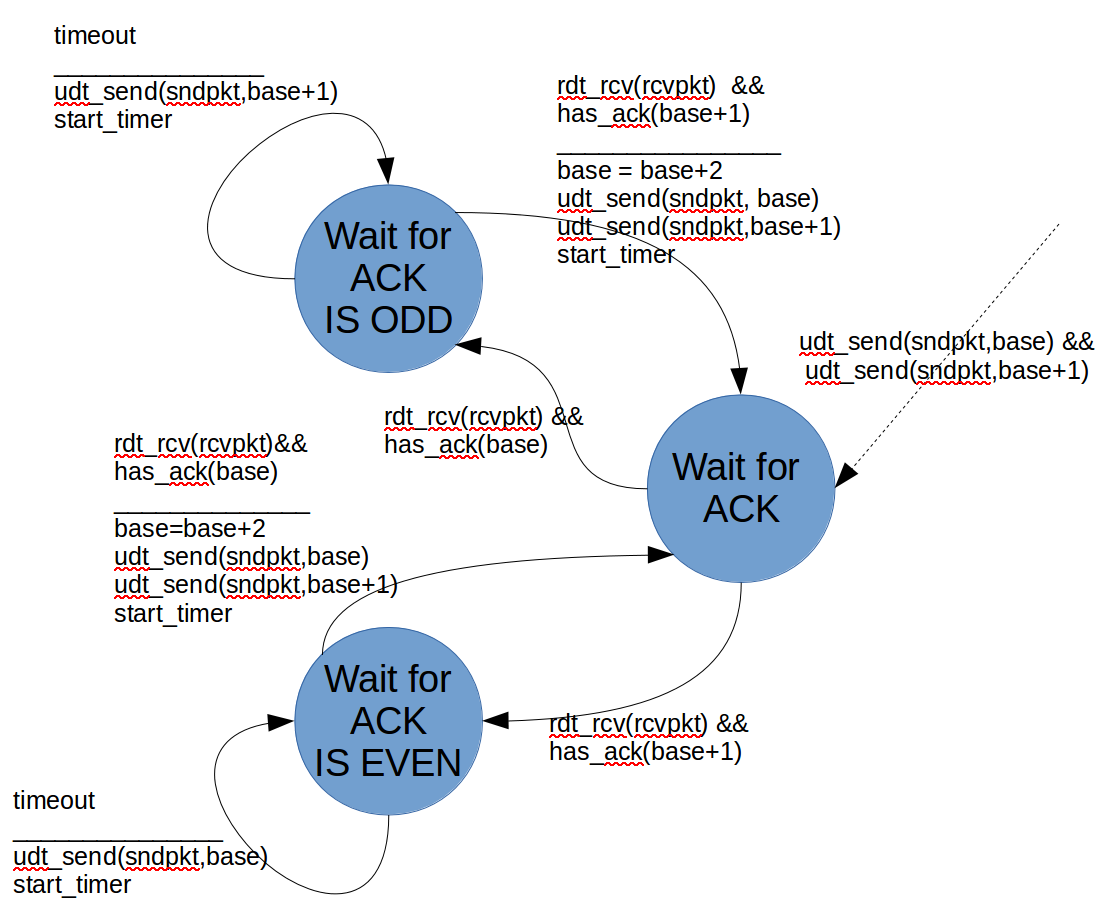
\includegraphics[width=\textwidth]{sender_18_fsm}
    DIAGRAM: \\
    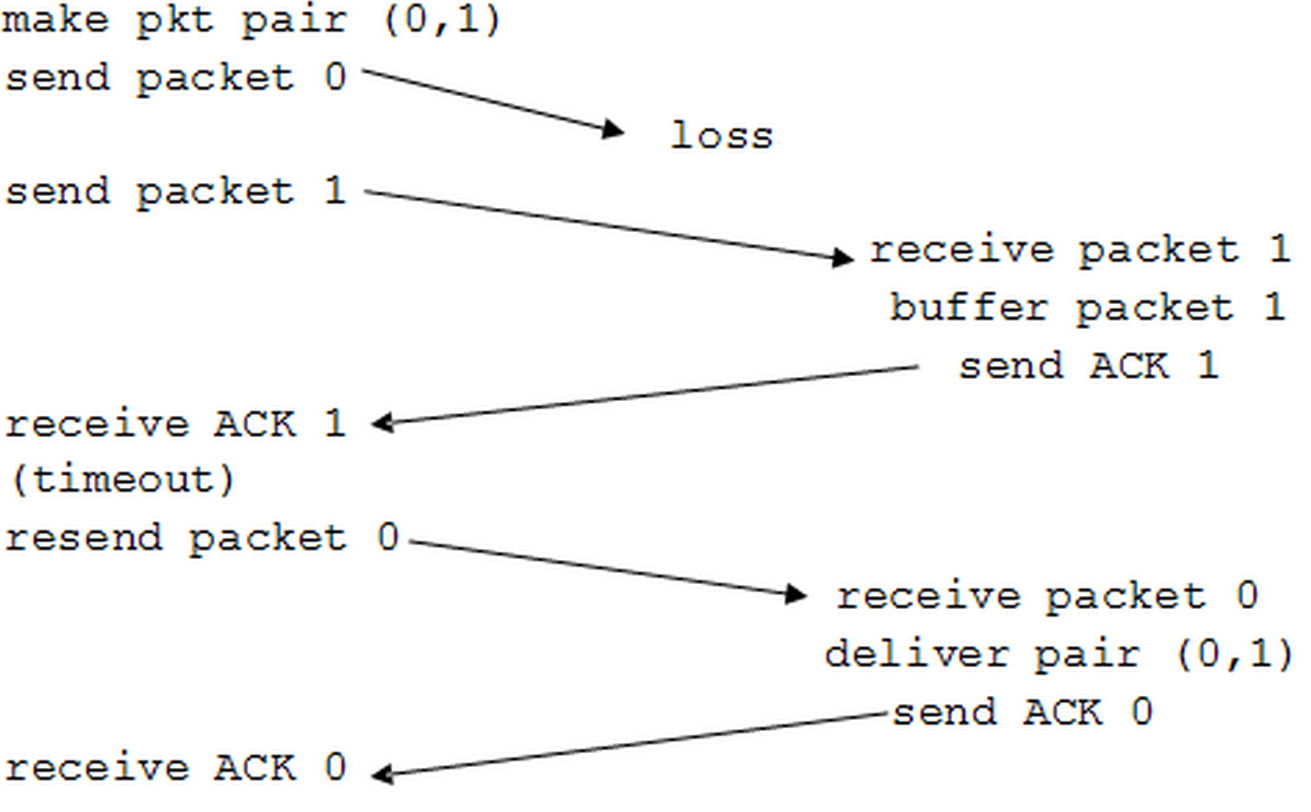
\includegraphics[width=\textwidth]{packet_Sending_diagram}


\item{Problem 3.22}
    \par
    A.The receiver has ACKED k-1 and  all the proceeding packets .If all the ACK has been received by the sender ,then the set is {k,k+1, k+2}. If all the ACK are lost, then the set is {k-3, k-2,k-1}   
    \\B.The receiver  is expecting the packet k, so the ACK of the proceeding packets must be sent to the receiver. If all the  former 3 ACK hasn't arrived at the sender ,then values of ACK includes k-1,k-2,k-3; since packet k-1 has been sent , the ACK of packet k-4 is no doubt that has got the sender so there are no ACK less than k-3 in the currently propagating back to the sender, neither ACK more than  or equal to k. \\
    Thus the possible values are {k-3,k-2,k-1}
    \pagebreak
\item{Problem 3.26}
    \par
    A )\\
    Given that the TCP sequence numer field is 4 bytes; \\
    $4bits*8bits=32bits$ \\
    Thus the possible sequence is $2^{32} \rightarrow 4294967296$ \\
    The MSS is irrelevant because the sequene is an incriment of the number of bytes sent. So then we can say that the file size between Host A and Host B is the number of bytes gien from  the equation of;\\
    $2^{32}\rightarrow2^2*2^{30}$ (all in bytes of course)\\
    The result of this equation is 4 Gigabytes.\\
    B )\\
    The number of segments is $\ceil{\frac{2^{32}}{536}}}$ where 536 is the max segment size given to us and the function is found in the book; the result of which is $8012999$\\
    The total number of bytes for different layer headers are added from each and every segment sent over the link; and so we are given $8012999*66=528857934$bytes in the header.\\
    Added to the number field, we get $2^{32}+528857934=4823825230\rightarrow4.824*10^9$bytes\\
    
    And using the transmit equation, we now get \\
    $\frac{4.824*10^9*8bits}{155*10^6bps\rightarrow}$\\
    $\frac{38592}{155}\rightarrow$\\
    $248.98$ seconds\\
\end{enumerate}

\end{document}
\documentclass[a4paper,11pt]{article}

\usepackage[T1]{fontenc}
\usepackage[utf8]{inputenc}
\usepackage{graphicx}
\usepackage{xcolor}

\renewcommand\familydefault{\sfdefault}
\usepackage{tgheros}
\usepackage[defaultmono]{droidmono}

\usepackage{amsmath,amssymb,amsthm,textcomp}
\usepackage{enumerate}
\usepackage{multicol}
\usepackage{tikz}
\usepackage{graphics}
\usepackage{lstlinebgrd}
\usepackage{color}
\usepackage{geometry}
\geometry{total={210mm,297mm},
left=25mm,right=25mm,%
bindingoffset=0mm, top=20mm,bottom=20mm}


\linespread{1.3}

\newcommand{\linia}{\rule{\linewidth}{0.5pt}}

\newtheoremstyle{mytheor}
    {1ex}{1ex}{\normalfont}{0pt}{\scshape}{.}{1ex}
    {{\thmname{#1 }}{\thmnumber{#2}}{\thmnote{ (#3)}}}

\theoremstyle{mytheor}
\newtheorem{defi}{Definition}

% my own titles
\makeatletter
\renewcommand{\maketitle}{
\begin{center}
\vspace{2ex}
{\huge \textsc{\@title}}
\vspace{1ex}
\\
\linia\\
\@author \hfill \@date
\vspace{4ex}
\end{center}
}
\makeatother
%%%

% custom footers and headers
\usepackage{fancyhdr}
\pagestyle{fancy}
\lhead{Page \thepage}
\chead{}
\rhead{Steven Seppala \& Seth Decker}
\lfoot{Programming assignment \textnumero{} 5}
\cfoot{Networks}
\rfoot{ECE 440}
\renewcommand{\headrulewidth}{0pt}
\renewcommand{\footrulewidth}{0pt}
%

% code listing settings
\usepackage{listings}
\lstset{
    language=[ANSI]C,
    basicstyle=\ttfamily\small,
    aboveskip={1.0\baselineskip},
    belowskip={1.0\baselineskip},
    columns=fixed,
    extendedchars=true,
    breaklines=true,
    tabsize=4,
    prebreak=\raisebox{0ex}[0ex][0ex]{\ensuremath{\hookleftarrow}},
    frame=lines,
    showtabs=false,
    showspaces=false,
    showstringspaces=false,
    keywordstyle=\color[rgb]{0.627,0.126,0.941},
    commentstyle=\color[rgb]{0.133,0.545,0.133},
    stringstyle=\color[rgb]{01,0,0},
    numbers=left,
    numberstyle=\small,
    stepnumber=1,
    numbersep=10pt,
    captionpos=t,
    escapeinside={\%*}{*)}
}
	\definecolor{dkgreen}{rgb}{0,0.8,0}
	\definecolor{gray}{rgb}{0.5,0.5,0.5}
	\definecolor{mauve}{rgb}{0.58,0,0.82}

%%%----------%%%----------%%%----------%%%----------%%%
%%%----------Document begins right below this-------%%%
%%%----------%%%----------%%%----------%%%----------%%%
\begin{document}

\title{Lab Problems \textnumero{} 1}

\author{Steven Seppala \& Seth Decker}

\date{30 October 2014}

\maketitle

\begin{center} \section*{Lab Problems} \end{center}

\begin{enumerate}
\item {Problem 3.17} \\
    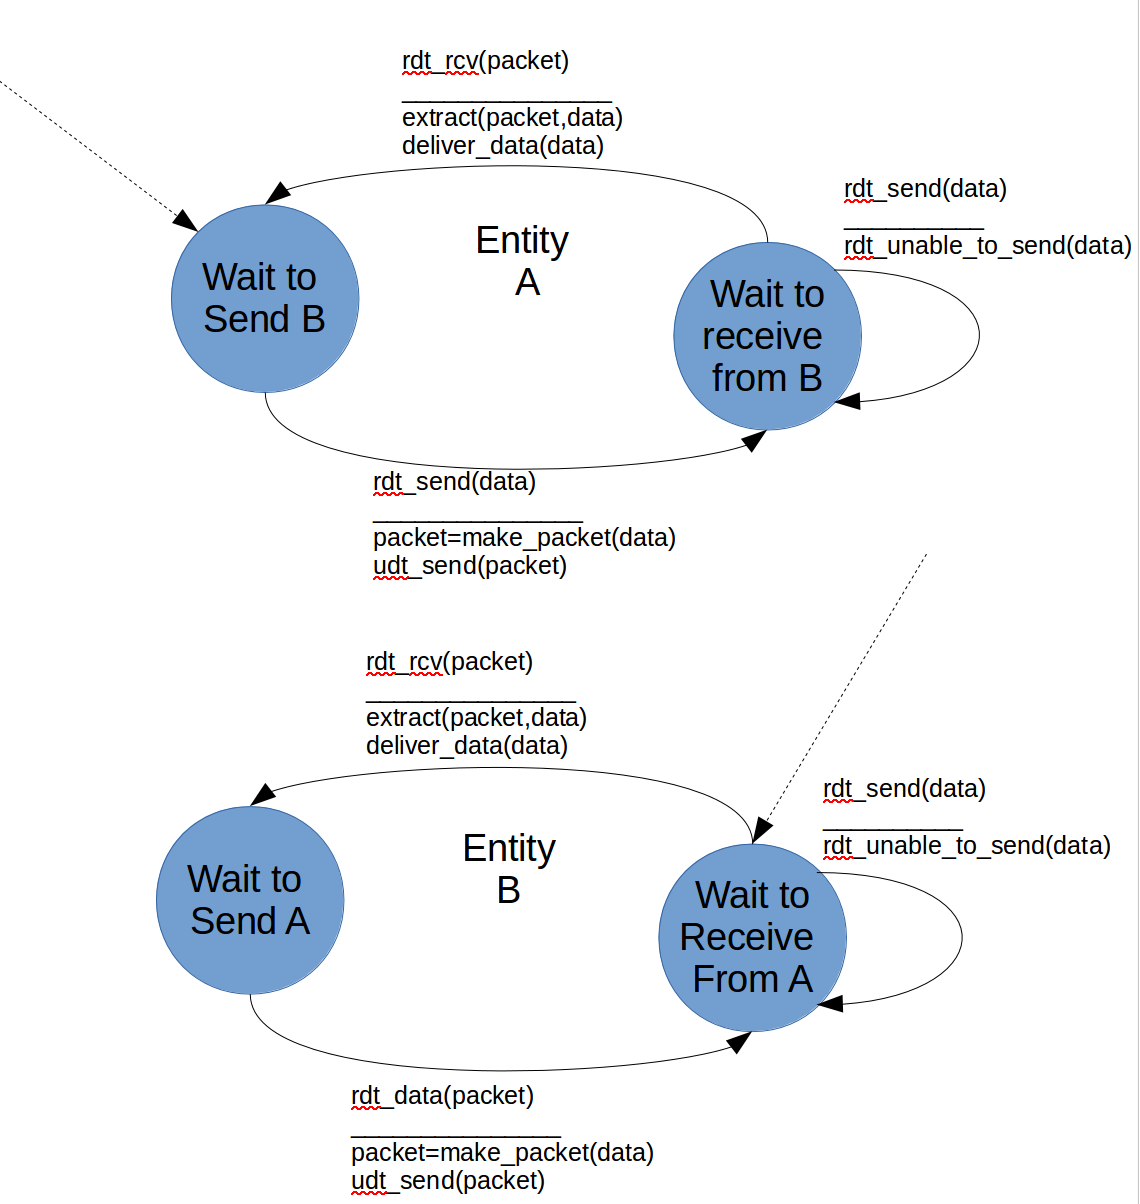
\includegraphics[width=120mm]{p17}\\
    Wait to recieve a packet and then extracts data and delivers it. And then waits for a signal to make and send a packet tot the next state.
    \pagebreak
\item{Problem 3.18}
    \par
    The sender waits for ACK before it can send the next pair of messages; the ACK messages received will have an ID that dictates which packet was received.\\
    The timer and timeout function use a timer to wait for a packet or for a delta T period.\\
    udt send function sends a packet with an acknowledgement ; base implies the even acknowledgement and base+1 implies odd acknowledgement.; has ack function implies that the received packet has the attached acknowledgement. ; udt send has a acknowledgement and a packet argument. \\
    RECIEVER: \\
    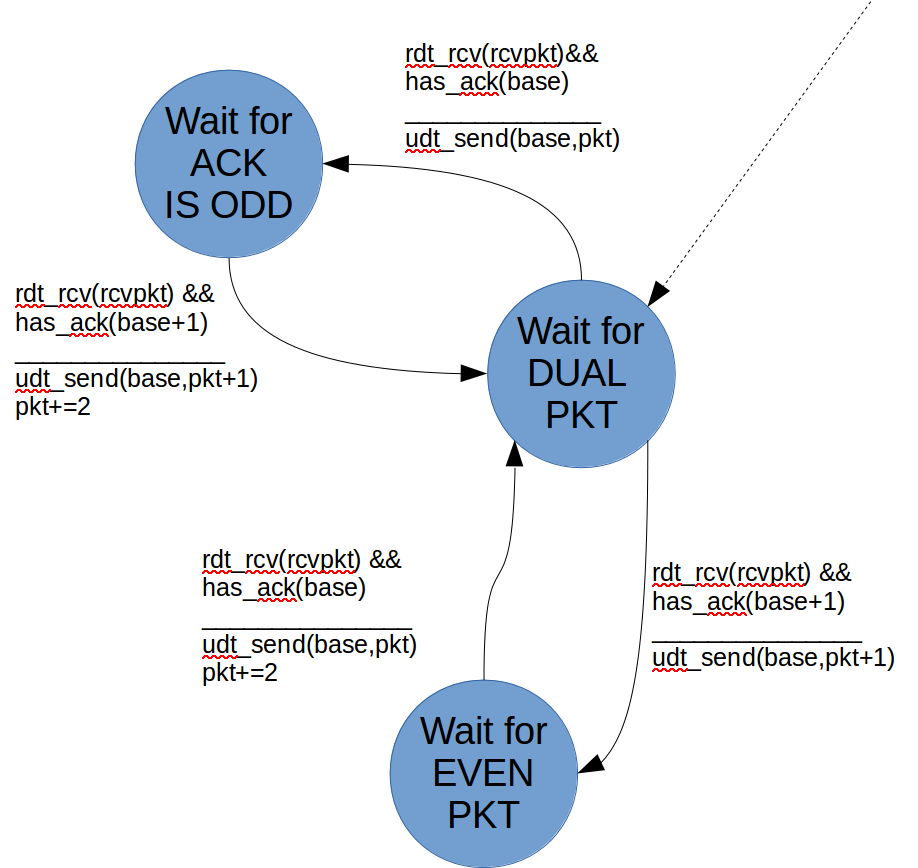
\includegraphics[width=\textwidth]{reciever_18_fsm}
    \pagebreak \\
    SENDER\\
    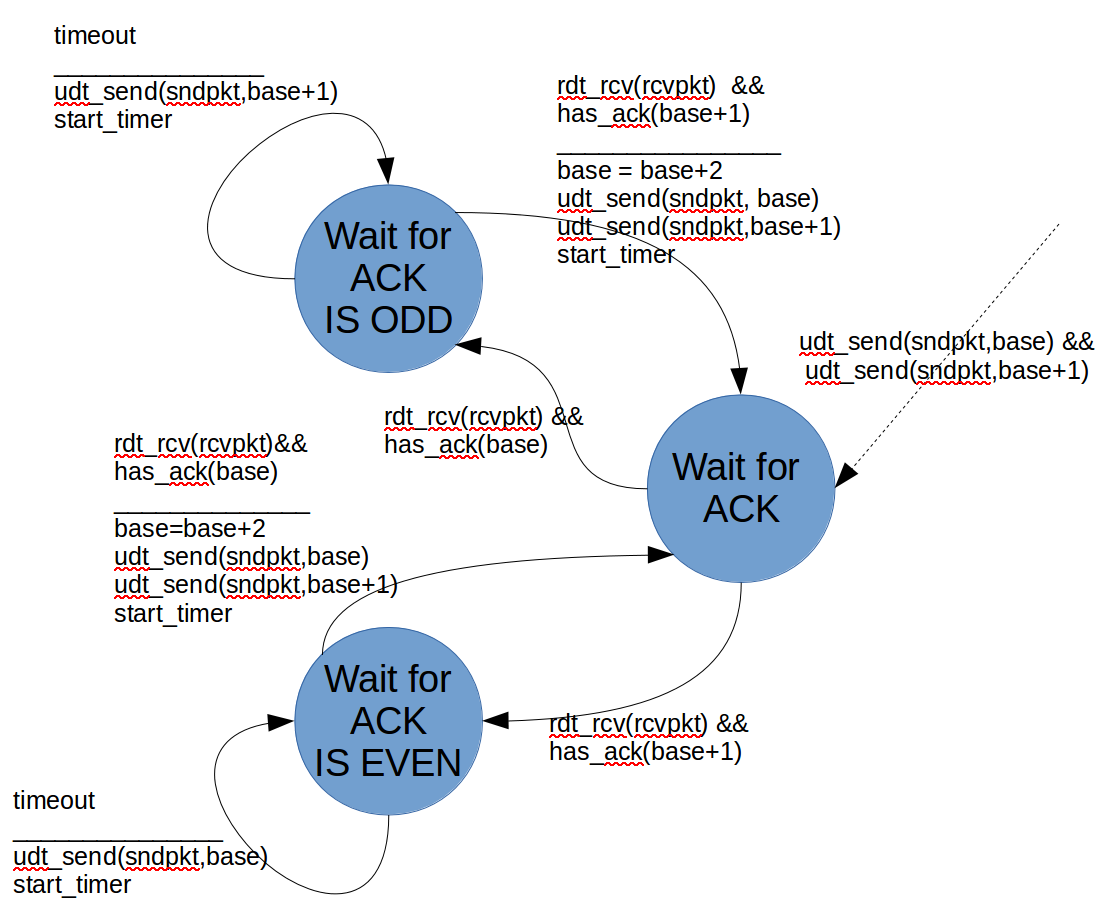
\includegraphics[width=\textwidth]{sender_18_fsm}
    \pagebreak \\
    DIAGRAM: \\
    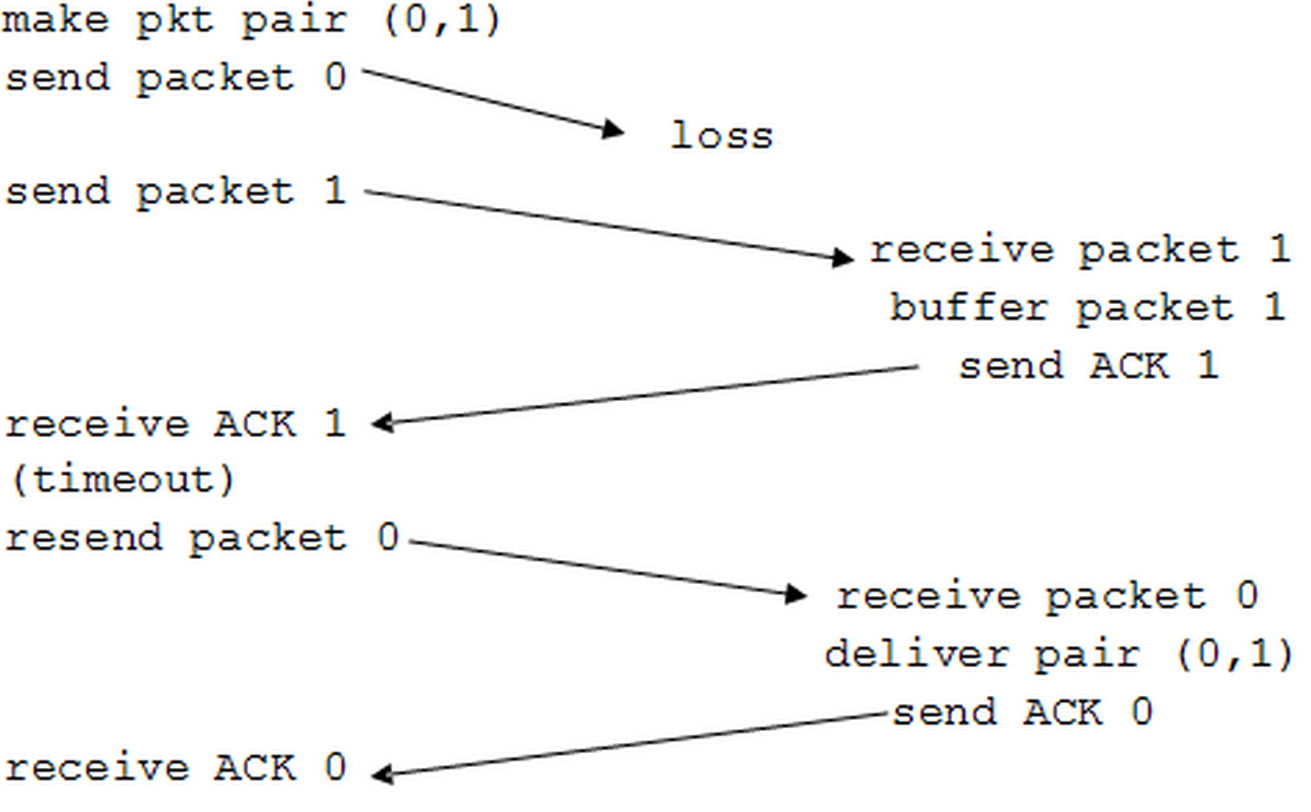
\includegraphics[width=\textwidth]{packet_Sending_diagram}
    \pagebreak
\item{Problem 3.22}
    \par
    A.The receiver has ACKED k-1 and  all the proceeding packets .If all the ACK has been received by the sender ,then the set is {k,k+1, k+2}. If all the ACK are lost, then the set is {k-3, k-2,k-1}   
    \\B.The receiver  is expecting the packet k, so the ACK of the proceeding packets must be sent to the receiver. If all the  former 3 ACK hasn't arrived at the sender ,then values of ACK includes k-1,k-2,k-3; since packet k-1 has been sent , the ACK of packet k-4 is no doubt that has got the sender so there are no ACK less than k-3 in the currently propagating back to the sender, neither ACK more than  or equal to k. \\
    Thus the possible values are {k-3,k-2,k-1}
\item{Problem 3.26}
    \par
    A )\\
    Given that the TCP sequence numer field is 4 bytes; \\
    $4*8bits=32bits$ \\
    Thus the possible sequence is $2^{32} \rightarrow 4294967296$ \\
    The MSS is irrelevant because the sequene is an incriment of the number of bytes sent. So then we can say that the file size between Host A and Host B is the number of bytes gien from  the equation of;\\
    $2^{32}\rightarrow2^2*2^{30}$ (all in bytes of course)\\
    The result of this equation is 4 Gigabytes.\\
    B )\\
    The number of segments is $\ceil{\frac{2^{32}}{536}}}$ where 536 is the max segment size given to us and the function is found in the book; the result of which is $8012999$\\
    The total number of bytes for different layer headers are added from each and every segment sent over the link; and so we are given $8012999*66=528857934$bytes in the header.\\
    Added to the number field, we get $2^{32}+528857934=4823825230\rightarrow4.824*10^9$bytes\\
    
    And using the transmit equation, we now get \\
    $\frac{4.824*10^9*8bits}{155*10^6bps\rightarrow}$\\
    $\frac{38592}{155}\rightarrow$\\
    $248.98$ seconds\\
\end{enumerate}

\end{document}
